\subsection{Usar el complemento de Python}

Escribir complementos en Python es mucho más sencillo que usar C++. Para crear un complemento de PyQGIS, 
necesita QGIS 0.9, Python, PyQt y las herramientas de desarrollo de Qt 
\cite{sherman07}.

Cuando QGIS arranca escanea ciertos directorios en busca de complementos tanto de C++ como de Python. 
Para que un archivo (biblioteca compartida, DLL o script de python) sea reconocido como complemento 
tiene que tener una firma específica. Para los scripts de Python es bastante sencillo. QGIS busca 
en las siguientes localizaciones dentro del directorio de instalación:

\begin{itemize}
\item \textbf{Linux y otros Unix}: ./share/qgis/python/plugins
\item \textbf{Mac OS X}: ./Contents/MacOS/share/qgis/python/plugins
\item \textbf{Windows}: .\textbackslash share\textbackslash QGIS\textbackslash
python\textbackslash plugins
\end{itemize}

Cada complemento de Python está contenido en su propio directorio. Cuando QGIS arranca busca en cada 
subdirectorio en \textsl{share/qgis/python/plugins} e inicializa cada complemento que encuentra. 
Una vez que esto está hecho, el complemento se mostrará en el administrador de complementos.

Vamos a crear un complemento para rellenar un hueco en la interfaz de QGIS. Esta complemento nos 
permitirá crear una nueva capa PostGIS para que la digitalicemos. Será un complemento sencillo y 
bastante burdo, pero ilustrará como iniciarse para escribir sus propios complementos de PyQGIS.

\subsubsection{Configurar la estructura}
Lo primero que necesitamos hacer es configurar la estructura de nuestro complemento. En
este ejemplo desarrollaremos nuestro complemento en Linux, pero el método es el mismo, 
solo que adaptado a las órdenes del sistema de archivos adecuados a su plataforma. 
QGIS está instalado en un directorio llamado \textsl{qgis\_09} dentro de su directorio 
personal. Vamos a crear el directorio para el complemento.

\begin{verbatim}
mkdir ~/qgis_09/share/qgis/python/plugins/capa_nueva
\end{verbatim}

Para empezar, necesitamos crear los siguientes archivos en el directorio \textsl{capa\_nueva}
  (necesitaremos algunos archivos adicionales dentro de poco):

\begin{verbatim}
__init__.py 
recursos.py
recursos.qrc
capanueva.py
\end{verbatim} 

\subsubsection{Hacer reconocible el complemento}

La inicialización del complemento se hace en el script \textsl{\_\_init\_\_.py}. Para nuestro 
complemento \textsl{CapaNueva} el script contiene:

\begin{verbatim}
1 # Cargar la clase CapaNueva desde el archivo capanueva.py
2 from capanueva import CapaNueva
3 def name():
4   return "Nueva capa PostGIS"
5 def description():
6   return "Crea una capa nueva Postgis vacía"
7 def version():
8   return "Version 0.1"
9 def classFactory(iface):
10   return CapaNueva(iface)
\end{verbatim} 

Las cosas que un complemento debe devolver de forma imperativa son un nombre, descripción y
versión, todo lo cual está implementado en nuestro script de arriba. Cada método simplemente 
devuelve una cadena con la información adecuada. El otro requisito es el método \textsl{classFactory} 
que debe devolver una referencia al propio complemento (línea 10), después de recibir el objeto 
\textbf{iface} como argumento. Con este sencillo código QGIS  reconocerá nuestro script como 
un complemento.

\subsubsection{Recursos}

Para poder tener un bonito icono para nuestro complemento, necesitamos un archivo de recursos
al que llamaremos \textsl{recursos.qrc}. Se trata de un sencillo archivo XML que define el 
recurso del icono:

\begin{verbatim}
 <RCC>
    <qresource prefix="/plugins/capanueva">
        <file>icono.png</file>
    </qresource>
</RCC> 
\end{verbatim} 

El archivo de recursos usa un prefijo para evitar conflictos con los nombres de otros complementos. 
Usar el nombre del complemento normalmente es suficiente. El archivo {icono.png} es simplemente una 
imagen PNG que se usará en la barra de herramientas cuando se active el complemento. Puede 
usar cualquier imagen con tal de que tenga 22x22 píxeles (para que se ajuste a la barra de herramientas).

Para convertir el archivo de recursos en algo que el complemento pueda usar, se debe compilar usando el compilador de recursos de PyQt:

\begin{verbatim}
  pyrcc4 -o recursos.py recursos.qrc
\end{verbatim}

El modificador \textsl{-o} se usa para especificar el archivo de salida. Ahora que tenemos recursos, 
necesitamos una forma de recoger la información necesaria para crear una capa nueva.

\subsubsection{Crear la interfaz gráfica de usuario (GUI)}

Normalmente usaríamos la misma herramienta que usan los desarrolladores de C++ para crear una GUI: Qt Designer. 
Se trata de una herramienta de diseño visual que le permite crear ventanas de diálogos y principales 
cogiendo y arrastrando herramientas y definiendo sus propiedades.

Para diseñar nuestro complemento CapaNueva podríamos conseguir herramientas bastante entretenidas e integradas 
para los tipos de campo y otras opciones. Sin embargo, puesto que nuestro tiempo es limitado, usaremos 
otros medios para recopilar la información que necesitamos para crear la tabla.
Esto ilustrará los 
conceptos y luego se podrá profundizar más usando los manuales del blog de QGIS.

Para recopilar la entrada del usuario, usaremos la clase \textsl{QInputDialog} de la biblioteca Qt. 
Esta pedirá al usuario una línea simple de entrada. Aunque esto hará nuestro complemento un poco 
crudo, servirá para ilustrar los conceptos.

Todo lo que tenemos que escribir ahora es el código de Python para recopilar la entrada y crear la tabla.

\subsubsection{Crear el complemento}

Una vez que tenemos los preliminares preparados podemos centrarnos en escribir el código que hará el trabajo real. 
Empezemos por mirar las cosas que necesitamos importar y la inicialización del complemento en \textsl{capanueva.py}.
 
\begin{verbatim}
1 # Importar las bibliotecas de PyQt y QGIS
2 from PyQt4.QtCore import *
3 from PyQt4.QtGui import *
4 from qgis.core import *
5 import psycopg
6 # Inicializar los recursos de Qt del archivo recursos.py
7 import recursos
8
9 # Nuestra clase principal para el complemento
10 class CapaNueva:
11
12  def __init__(self, iface):
13    # Guardar la referencia para la interfaz de QGIS
14    self.iface = iface
15
16  def initGui(self):
17    # Crear la acción que iniciará la configuración del complemento
18    self.action = QAction(QIcon(":/plugins/capa_nueva/icono.png"),\
19      "Nueva capa PostGIS", self.iface.getMainWindow())
20    QObject.connect(self.action, SIGNAL("activated()"), self.run)
21
22    # Añadir botón a la barra de herramientas y entrada del menú
23    self.iface.addToolBarIcon(self.action)
24    self.iface.addPluginMenu("&Nueva capa PostGIS...", self.action)
25
26  def unload(self):
27    # Eliminar la entrada del menú y el icono del complemento
28    self.iface.removePluginMenu("&Nueva capa PostGIS...",self.action)
29    self.iface.removeToolBarIcon(self.action)
\end{verbatim}

En las líneas 2 a 7 importamos las bibliotecas necesarias para el complemento. Esto incluye las bibliotecas 
de PyQt, la biblioteca principal de QGIS y la biblioteca de Python 
PostgreSQL psycopg. 
Cada script de Python que use las bibliotecas de QGIS y PyQt necesita importar las bibliotecas de QtCore 
y QtGui, así como la biblioteca principal de QGIS. Esto nos da acceso a los PyQt wrappers para nuestros 
objetos de Qt (como nuestro diálogo de entrada) y la biblioteca principal de QGIS. 
También necesitamos importar el archivo \textsl{recursos.py} que creamos con la definición del icono.

En la línea 10 declaramos la clase \textbf{CapaNueva}. En el método \textsl{\_\_init\_\_} 
(líneas 12 a 14) se inicializa nuestra clase y se pasa el objeto \textbf{iface} de QGIS via el método 
\textsl{classFactory} en la línea 10 de \_\_init\_\_.py. Guardamos \textbf{iface} como 
una variable de miembro, de forma que la podamos usar después.

En las líneas 16 a 24 inicializamos los elementos de la GUI para el complemento. En Qt se usa una 
\textbf{QAction} para crear una acción de la interfaz de usuario que se puede usar para crear tanto 
un elemento de menú como de la barra de herramientas. En nuestro complemento lo usamos para ambas cosas. 
En la línea 18 creamos la acción usando nuestro recurso de icono (observe el prefijo que hemos especificado 
en \textsl{recursos.qrc}). También proporcionamos algo de texto que aparecerá cuando se use en un menú o al 
pasar el ratón por encima y finalmente necesitamos especificar el ``padre''. En un complemento, el padre es 
la ventana principal de QGIS. El objeto \textbf{iface} que guardamos durante la inicialización nos permite 
obtener la referencia a la ventana principal en la línea 19.

Una vez que la acción está creada, podemos añadirla tanto a la barra de herramientas como al menú 
de \textsl{Complementos} (líneas 23 y 24). Esto se encarga de inicializar la GUI para el complemento. La otra 
cosa que necesitamos es hacer limpieza detrás nuestra cuando se descarga el complemento. El método 
\textsl{unload} se encarga de esto eliminando la entrada del menú y la herramienta de la barra de herramientas (líneas 28 y 29).

Esto se encarga del proceso de inicialización y de que nuestro complemento se cargue y descargue correctamente. 
Miremos ahora al código que hace el verdadero trabajo. Todo se encuentra en el método \textsl{run}.

\begin{verbatim}
30 def run(self): 
31   # Obtener la entrada del usuario, comenzando por el nombre de la tabla
32   table_name = QInputDialog.getText(None, "¿Nombre de la tabla?", \
33     "Nombre para la nueva capa PostGIS")
34   if table_name[0].length() > 0:
35     # Obtener los nombres y tipos de los campos
36     fields = QInputDialog.getText(None, "Nombres de los campos", \
37      "Campos (separados por coma)")
38     parts = fields[0].split(',')
39     # Crear la sencencia SQL
40     sql = "create table " + table_name[0] + " (id int4 primary key, "
41     for fld in parts:
42      sql += fld + " varchar(10), "
43     sql = sql[0:-2]
44     sql += ")"
45     # Conectar con la base de datos
46     # Primero obtener la DSN
47     dsn = QInputDialog.getText(None, "DSN de la base de datos", \
48      "Introducir la DSN para conectar con la base de datos (dbname=db user=user)")
49     if dsn[0].length() > 0:
50      con = psycopg.connect(str(dsn[0]))
51      curs = con.cursor()
52      curs.execute(str(sql))
53      con.commit()
54      # añadir la columna de la geometría
55      curs.execute("select AddGeometryColumn('" + str(table_name[0]) + \
56        "', 'the_geom', 4326, 'POLYGON', 2)")
57      con.commit()
58      # crear el índice GIST
59      curs.execute("create index sidx_" + str(table_name[0]) + " on " + \
60        str(table_name[0]) + " USING GIST(the_geom GIST_GEOMETRY_OPS)")
61        con.commit()
\end{verbatim}

Lo primero que tenemos que hacer es usar \textbf{QInputDialog} para obtener el nombre de la tabla a crear. 
Esto se hace en la línea 32, en la que se pide el nombre.

\begin{figure}[ht]
\begin{center}
  \caption{Introducir nombre de la nueva tabla PostGIS}\label{fig:gettablename}\smallskip
  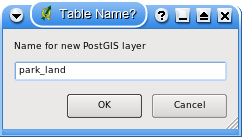
\includegraphics[scale=0.8]{gettablename}
\end{center}
\end{figure}

En la línea 34 comprobamos que el usuario realmente ha introducido algo antes de continuar.

A continuación necesitamos obtener los nombres de los campos. Para este ejemplo lo vamos a hacer muy simple. 
Cada campo será un varchar(10), lo que significa que puede almacenar hasta 10 caracteres. Si realmente queremos 
hacer útil este complemento, necesitaremos proporcionar una forma de que el usuario especifique el tipo. En 
la línea 36 pedimos al usuario que introduzca una lista de nombres de campos separados por comas.

\begin{figure}[ht]
\begin{center}
  \caption{Introducir nombres de campos para la nueva tabla PostGIS}\label{fig:getfieldname}\smallskip
  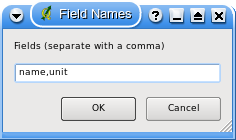
\includegraphics[scale=0.8]{getfieldname}
\end{center}
\end{figure}

Luego dividimos esta lista en sus componentes para usarla en la construcción de la sentencia (línea 38). 

La línea 40 contiene la primera parte de la sentencia SQL. Observe que estamos creando la tabla con un campo 
ID entero que será la clave primaria. A continuación iteramos por la lista de campos, añadiendo el código 
adecuado a la sentencia SQL (línea 41).

Una vez que tenemos todos los campos añadidos a la sentencia SQL, truncamos los caracteres de trailing que no 
queremos (línea 43) y luego añadimos el paréntesis de cierre para completar la sentencia (línea 44).

Ahora ya estamos preparados para conectar a la base de datos y crear la tabla. Para acceder a la base de datos 
usamos psycopg (\url{http://www.initd.org}). Para poder conectar a la base de datos tenemos que especificar 
el nombre de la fuente de datos (DSN-Data Source Name) con el nombre de la base de datos, usuario y contraseña 
si es necesario. Si estamos ejecutando tanto QGIS como PostgreSQL en la misma máquina normalmente no es 
necesario especificar una contraseña. En este caso, el DSN tendrá un aspecto parecido a esto:

\begin{center}
  \textsl{dbname=gis\_data user=gsherman}
\end{center}

Para obtener el DSN, preguntamos a usuario con un \textbf{QInputDialog} en la línea 47.

\begin{figure}[ht]
\begin{center}
  \caption{Introducir DSN para la conexión a la base de datos PostGIS}\label{fig:getdsn}\smallskip
  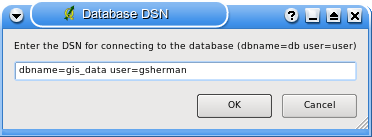
\includegraphics[scale=0.8]{getdsn}
\end{center}
\end{figure}

Si el usuario introduce un DSN podemos continuar con la conexión a la base de datos en la línea 50. Obtenemos 
el cursor desde la conexión en la línea 51 y luego ejecutamos la sentencia SQL para crear la tabla y remitir 
el cambio en las líneas 52 a 53. Esto crea la tabla, pero para que ésta sea una capa válida y lista para usarla, 
necesita un par de cosas más. 

Primero necesita una columna de geometría. No hemos introducido una a propósito cuando creamos la tabla para 
poder usar la función \textsl{AddGeometryColumn} para crearla. Esta función añade una columna de geometría 
y luego pone una entrada en la tabla \textsl{geometry\_columns} por nosotros. En 
la línea 55 especificamos el 
nombre de la tabla, el nombre que queremos para la columna de geometría, el SRID, tipo de objeto espacial 
y sus dimensiones.

Lo último que hay que hacer es crear el índice espacial en la tabla, de forma que obtengamos un funcionamiento 
óptimo cuando hagamos búsquedas espaciales y mostremos los datos en QGIS. En la línea 59 hemos apañado junta la 
SQL para crear el índice. La sentencia real es la siguiente:

\begin{verbatim}
create index sidx_park_land on park_land 
   USING GIST(the_geom GIST_GEOMETRY_OPS);
\end{verbatim}

\subsubsection{Fallos y problemas}

Nuestro complemento ya está completo. Veamos ahora algunas cosas que están mal en él o que podemos mejorar:

\begin{itemize}
\item Podríamos usar una GUI mejorada, una que permita al usuario introducir toda la información necesaria en un diálogo.
\item El usuario no puede especificar tipos de campos.
\item La comprobación de errores es limitada en el diálogo.
  \begin{itemize}
    \item Si no se introduce ningún campo el complemento falla.
    \item No hay comprobación de errores en ninguna de las operaciones de base de datos.
  \end{itemize} 
\item No hay retroalimentación desde el complemento una vez que finaliza.
\end{itemize} 

A pesar de todos estos fallos, aún sirve como un complemento primordial que ilustra el proceso y ayuda 
a iniciarse en el desarrollo de complementos.

\subsubsection{Añadir retroalimentación}

Vamos a solucionar uno de los pequeños problemas añadiendo algo de retroalimentación al final del 
proceso. Sólo añadiremos un cuadro de mensaje para indicar al usuario que todo está hecho y para comprobar 
la base de datos para asegurarnos de que se creó la tabla.

Para hacer esto, simplemente añadiremos el siguiente código después de la línea 61:

\begin{verbatim}
# mostrar al usuario lo que ha ocurrido
QMessageBox.information(None, "Resultados", "La tabla " + str(table_name[0]) + \
" se ha creado. Compruebe su base de datos para confirmar.")
\end{verbatim}

Cuando la tabla se cree el usuario verá esto:

\begin{figure}[ht]
\begin{center}
  \caption{Cuadro de mensaje con los resultados del complemento}\label{fig:plugin_results}\smallskip
  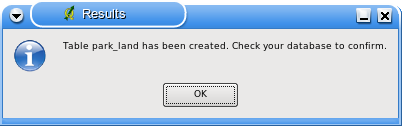
\includegraphics[scale=0.8]{plugin_results}
\end{center}
\end{figure}

\subsubsection{Resumen}
Escribir un complemento de QGIS en Python es bastante sencillo. Algunos complementos no requerirán 
siquiera una GUI. Por ejemplo, podría escribir un complemento que devuelva las coordenadas del mapa para el 
punto del mapa en el que pulse. Tal complemento no requeriría ninguna entrada por parte del usuario y podría 
usar un \textbf{QMessageBox} estándar de Qt para mostrar el resultado.

También puede escribir complementos para QGIS en C++, paro eso es otra historio. Puede encontrar manuales sobre 
la escritura de complementos de QGIS tanto en C++ como en Python en el blog de QGIS en:

\begin{center}
  \url{http://blog.qgis.org} 
\end{center}

% vim:tw=76:autoindent